\subsubsection{Allgemeine Informationen zu der Richtlinie}
Auf Basis der in der Balkenberechnung bestimmten Parameter Biegesteifigkeit, maximales Biegemoment und maximale Querkraft, werden die Gurte und der Steg dimensioniert. Die Vorauslegung erfolgt dabei anhand der VDI-Richtlinie 2013 \cite{item5}. Diese behandelt die Dimensionierung von GFK-Teilen und enthält in einem Unterkapitel Informationen speziell zur Auslegung eines I-Trägers. Zur Festigkeitsauslegung werden die Gurte und der Steg getrennt voneinander betrachtet. Es wird die Annahme gemacht, dass der Gurt unter Vernachlässigung der Schubflussaufnahme das gesamte Biegemoment aufnehmen soll. Der Steg hingegen wird, neben einem über die Höhe konstanten Schubfluss, auch durch die aufgeprägte Deformation der Gurte beansprucht. Das orthotrope Werkstoffverhalten des Laminats, sowie die Festigkeitseigenschaften bei verschiedenen Beanspruchungen, werden allein durch die "charakteristischen K-Werte" \cite{item5} berücksichtigt. Diese wurden in Untersuchungen an GFK-Proben für Rovings und Gewebe ermittelt und tabelliert \cite{item5}. Auf diese Weise erlauben die Berechnungen der Richtlinie keine Aussagen über resultierende Versagensformen in einzelnen Schichten. Die vorangestellte Auslegung der Gurte ist in dieser Form nicht Teil der Richtlinie. Um die Anforderungen an die Steifigkeit der Tragfläche zu erfüllen, ist die Analyse der Flächenträgheitsmomente jedoch unumgänglich. 
Zusätzlich sei angemerkt, dass kapitelübergreifend die gesamte Auslegung nur an ausgewählten und speziell gekennzeichneten Stellen Sicherheitsfaktoren ungleich eins berücksichtigt. Grund dafür ist die Annahme, dass in den bereitgestellten Materialkennwerten ausreichende Sicherheiten verrechnet worden sind. 
Die Vorauslegung hat den Anspruch, die Grundlagen für die aufbauende Berechnung mithilfe eines Laminatrechners zu legen.

\subsubsection{Dimensionierung der Gurte mit rechteckigen Querschnitten}
\label{GurtDim} 
Im ersten Auslegungsschritt der schubstarren Gurte wird die Einhaltung der Anforderungen an die Steifigkeit betrachtet.   
Die in der Balkenberechnung ermittelte Biegesteifigkeit $ EI_{x} = 962,552 Nm^{2} $, die erforderlich ist, damit bei einer Kraft $ F_{pruef}=100N $ die Flügelspitze eine Absenkung von $ w_{j=1,1}=20mm $ erfährt, muss, wegen oben genannter Annahme, allein durch die Gurte aufgebracht werden. Im Sinne der kraftflussgerechten Gestaltung sollen die Glasfasern unidirektional in Längsrichtung des Gurtes angeordnet werden. Die Bezeichnungen der Längenangaben des Holms orientieren sich an Abbildung~\ref{fig: Rechteckholm}~.\\

\begin{figure}[h]
	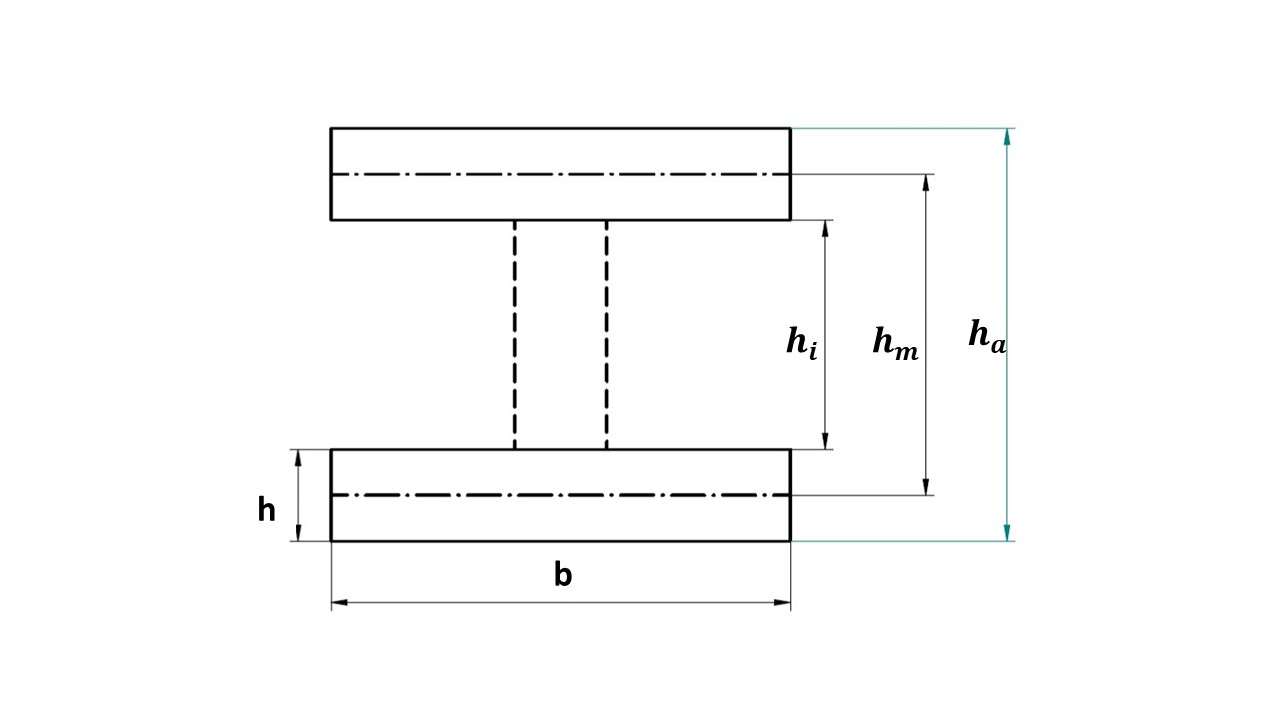
\includegraphics[width=1.0\textwidth]{Bilder/RechteckHolm.jpg}
	\caption{Bezeichnungen des I-Holms}
	\label{fig: Rechteckholm}
\end{figure}

\noindent Die Gurtquerschnitte werden zur Bestimmung der notwendigen Lagenanzahl als rechteckig angenommen, erst in einem späteren Schritt soll die Form dem vorgegebenen Hautprofil angepasst werden. Die Maße sind über die gesamte Länge des Holms in y-Richtung als konstant anzusehen.\\
Zur Bestimmung des Flächenträgheitsmoments $ I_{x} $ wird der E-Modul in Längsrichtung der Fasern gemäß der Mischungsregel nach \cite{item3} berechnet.\\
\begin{equation}
 E_{11}=  \varphi\cdot E_{f,11}+\left( 1-\varphi \right) \cdot E_{M}
\end{equation}
Mit den gegebenen Materialkennwerten $ E_{f,11}=74000MPa $, $ E_{m}=3300MPa $ und $ \varphi=0,4 $ bestimmt sich $ E_{11} = 31580 MPa $. Damit ergibt sich ein benötigtes Flächenträgheitsmoment von 
\begin{equation}
	I_{x,min} = \frac{962,552Nm^{2}}{31580\cdot 10^{6}Pa} =3,0479 \cdot 10^{-8} m^{4}
\end{equation}

\noindent Das Flächenträgheitsmoment der Gurte bestimmt sich aus den Flächenträgheitsmomenten der beiden Rechteckquerschnitte und ihren zugehörigen Steiner-Anteilen, die aus der Verschiebung der Gurte um jeweils $ \frac{h_{m}}{2} $ in z-Richtung resultieren. Da die Gurtdicke noch nicht bekannt ist, wird auf die Annahme der Gurte als "punktförmige Flächen" \cite{item15} verzichtet und der Eigenanteil mitbetrachtet. 
\begin{equation}
	\label{Ix}
	I_{x}=2\cdot\left(\frac{b\cdot h^{3}}{12}+b\cdot h\cdot\left(\frac{h_{m}}{2}\right)^{2}\right)
\end{equation}

\noindent Es wird nach einer Kombination aus Gurtbreite $ b $ und Gurthöhe $ h $ gesucht, die die Anforderungen an das Flächenträgheitsmoment erfüllt, aber dennoch zu einer möglichst geringen Gurtquerschnittsfläche und damit zu einer möglichst geringen Masse der Gurte führt. Um die Steiner-Anteile der Gurte zu maximieren, sollen die Gurte in einem möglichst großen Abstand zur neutralen Faser angeordnet werden. Gemäß der gegebenen technischen Zeichnung der Profilkontur, lässt sich das Profil von einem Rechteck der Höhe $ 37,5mm $ umrahmen. Dies entspricht jedoch nicht der Profildicke, da die Punkte mit dem größten Abstand zur Profilsehne auf der Ober- und Unterseite bei verschiedenen Flügeltiefen vorliegen. Zusätzlich muss oberhalb und unterhalb der Gurte ein Freiraum für die umliegenden Haut berücksichtigt werden. Deshalb wird die gesamte Gurthöhe auf $ h_{a}=36mm $ abgeschätzt. Die dadurch begrenzte Anzahl der Lagen in der Haut wird im Kapitel \ref{CAD} weiter erläutert.\\ 

\noindent Die folgende Übersicht enthält Werte der Gurtquerschnittsfläche bei verschiedenen Kombinationen von $ b $ und $ h $, die zum erforderlichen gesamten Flächenträgheitsmoment von $ I_{x,min} = 3,0479 \cdot 10^{-8} m^{4} $ führen.\\

		\begin{tabular}{l|c|r}
			$h$&$b$&$2\cdot b\cdot h$\\
			\hline
			$1mm$&$38,3mm$&$76,6mm^{2}$\\
			$1,25mm$&$31,1mm$&$77,7mm^{2}$\\
			$1,5mm$&$26,3mm$&$78,8mm^{2}$\\
			$2,25mm$&$18,3mm$&$82,3mm^{2}$\\
		\end{tabular}\\

\noindent Den Daten ist zu entnehmen, dass breite Gurte geringer Dicke bei gleichem Flächenträgheitsmoment geringere Querschnittsflächen aufweisen. Aus diesem Grund sollen die Gurte möglichst breit gewählt werden. Die Breite der Gurte ist durch die vorgegebene Konstruktion der Platte zur Aufnahme der Tragfläche am Teststand begrenzt. Die vorgesehene Aussparung weist eine Breite von $ 30mm $ auf. Für die weitere Berechnung soll $ b=28mm $ gelten. Diese Annahme wird dadurch begründet, dass die Fertigung des Holms im Bereich des Modellbaus von Hand erfolgen würde, womit nur grobe Toleranzen einhaltbar sind.
Mithilfe eines Solvers bestimmt sich aus dem Flächenträgheitsmoment und der Gurtbreite die Gurthöhe $ h=1,866mm $.\\
\noindent Im nächsten Schritt wird die zu stapelnde Lagenanzahl ermittelt. Als vorwiegend unidirektionales Material steht das Glasfasergewebe Interglas 92145 mit einem Flächengewicht von $ 220\frac{g}{m^{2}} $ zur Verfügung. Laut Produktdatenblatt \cite{item17} handelt es sich um eine Leinwandbindung, die eine nicht angegebene, da sehr kleine, Zugfestigkeit in Schussrichtung aufweist. Folgend wird das Gewebe als unidirektional behandelt. Nach \cite{item3} berechnet sich die Lagenanzahl $ n $ für eine Dicke des Verbundes $ t_{soll} $ zu:\\

\begin{equation}\label{Dicke}
	n=t_{soll}\cdot \frac{\varphi\cdot\rho_{f}}{\left(\frac{m_{f}}{L\cdot b}\right)}.
\end{equation}

\noindent Mit $ \left(\frac{m_{f}}{L\cdot b}\right) = 220\frac{g}{m^{2}} $, $ t_{soll}=h $ und $ \rho_{f}=2550\frac{kg}{m^{3}} $ ergibt sich $ n=8,653 $. Es sind also 9 Lagen des Gewebes 92145 für jeden Gurt vorzusehen.Die sich aus 9 Lagen ergebende Gurthöhe kann durch Umstellen von Gleichung ~\ref{gurtlagen} zu $ \tilde{h}=1,941mm $ bestimmt werden. Für den zunächst angenommenen Fall von Gurten mit rechteckigen Querschnitten ist die Auslegung zur Einhaltung der Anforderungen an die Steifigkeit damit abgeschlossen.\\


\subsubsection{Nachrechnung der angepassten Gurte} \label{NachrechnungGurte}
 Die Modellierung der Haut und der Holmgurte in einem CAD-Programm zeigt, dass die Gurte mit den berechneten Bemaßungen nicht innerhalb des Profils mit einer vorläufigen, als $ 0,75mm $ dick angenommenen Haut liegen. Die Anpassung der Konstruktion der Gurte erfolgt so, dass die Gurtaußenseite an der Innenseite der Haut anliegt (vgl. Abschnitt \ref{GurtKonstrukt}). Die Gesamtbreite von $ 28mm $, sowie die Gurtdicke $ h $ bleiben dabei erhalten. Die Gesamthöhe $ h_{a} $ muss auf $ \tilde{h}_{a}=35,8mm $ leicht verringert werden. Abbildung ~\ref{fig: KrummerGurt} veranschaulicht die gekrümmte Form des oberen Holmgurtes.
 \begin{figure}[h]
 	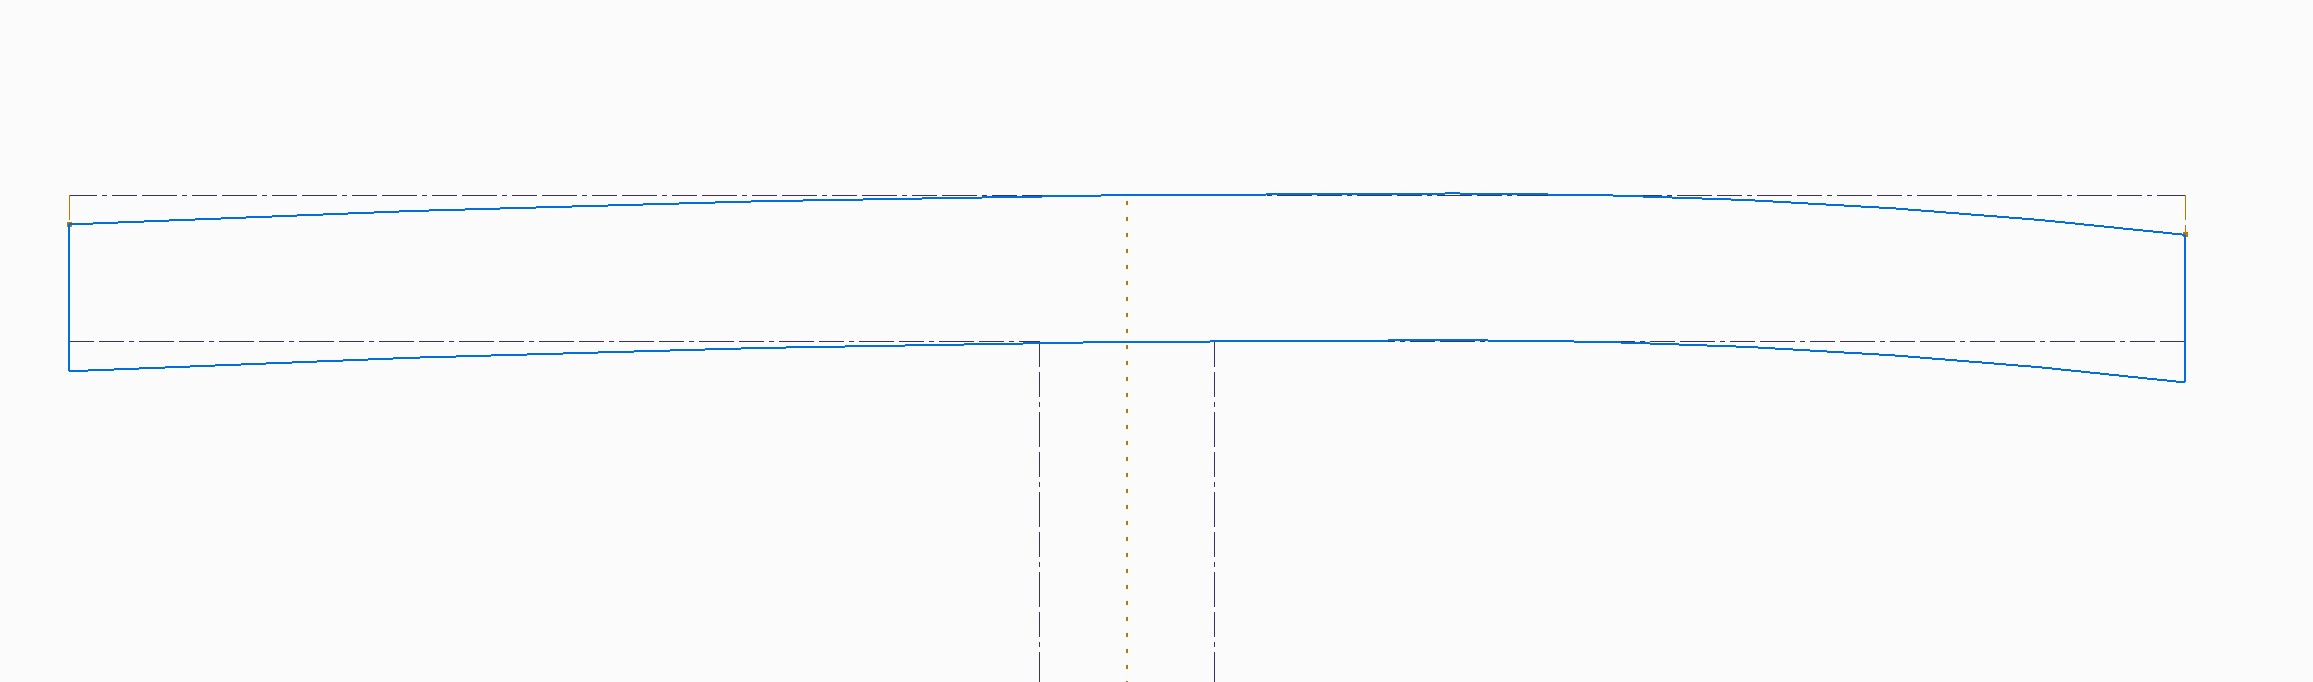
\includegraphics[width=1.0\textwidth]{Bilder/KrummerGurt.jpg}
 	\caption{Angepasste gekrümmte Gurtkontur}
 	\label{fig: KrummerGurt}
 \end{figure}

\noindent Die angepasste Krümmung der Gurte führt zu einem veränderten Flächenträgheitsmoment $ \tilde{I_{x}} $ des Balkens, dass mithilfe des CAD-Programms zu $ \tilde{I_{x}}=3,075406\cdot 10^{-8}m^{4} $ bestimmt werden kann. Da 
\begin{equation}
	\label{IVergleich}
	\tilde{I_{x}}=3,075406\cdot 10^{-8}m^{4} > I_{x,min}=3,0479\cdot 10^{-8}m^{4}
\end{equation}
gilt, genügen auch die veränderten Gurte der Steifigkeitsanforderung.\\
 
\noindent Abschließend wird gezeigt, dass die Festigkeit der Gurte einer Belastung der Flügelspitze durch $ F_{pruef}=500N $ standhält. Die aus der Biegung resultierenden und betragsmäßig gleichen Zug- und Druckspannungen werden dazu mit den gegebenen UD-Festigkeitskennwerten des Handlaminats verglichen. Die Resultate der Balkenberechnungen zeigen, dass das maximale Biegemoment im Holm an Punkt C auftritt und $ M_{b}=500N\cdot 0,773m=386,5Nm $ beträgt. In den Randfasern der Gurte resultieren Spannungen, die sich gemäß \cite{item15} zu\\
\begin{equation}
	\sigma_{b}=\frac{M_{b}\cdot \tilde{h}_{a}}{\tilde{I_{x}}\cdot 2}=224,96MPa
\end{equation} 
berechnen. Da 
\begin{equation}
	\sigma_{b}< R^{(+)}_{||}=597,9 MPa < |R^{(-)}_{||}| =650,0 MPa
\end{equation} 
gilt, ist der Festigkeitsnachweis erbracht. Es kann davon ausgegangen werden, dass die Gurte bei einer Prüfkraft von $ F_{pruef}=500N $ nicht versagen. \\

\subsubsection{Bestimmung der Lagenanzahl des Steges}
Bei der Auslegung des Steges muss beachtet werden, dass der Steg sowohl durch Schubkräfte als auch durch Normalkräfte senkrecht und parallel zu den Gurten Belastungen erfährt. Die Dehnungen Gurtinnenseiten werden dem Steg aufgeprägt, da beide Bauteile stoffschlüssig miteinander verbunden sind. Anders als in der VDI 2013 wird jedoch nicht die Bruchdehnung in der Gurtmittelebene betrachtet, sondern die Dehnungen der Innenseiten bei einer Prüfkraft von 500N. So soll die Dimensionierung des Steges auf die Anforderungen an die Festigkeit angepasst werden, um eine Überdimensionierung zu vermeiden. Im Folgenden bezeichnen $ n_{\epsilon}, n_{A} $ und $ q_{s} $ Kraftflüsse, $ n $, ohne einen Index, die Lagenanzahl und $ \bar{q} $ das Flächengewicht (in Newton) des trockenen Gewebes.\\

\noindent Die größte Längsdehnung der Gurte tritt an der Stelle C auf, da dort das größte Biegemoment wirkt. Sie lässt sich für die Innenseiten der Gurte nach \cite{item16} durch
\begin{equation}
	\epsilon_{Gurt}=\frac{\sigma_{innen}}{E_{11}}=\frac{\frac{F_{pruef}\cdot l_{3}\cdot h_{i}}{\tilde{I}_{x}\cdot 2}}{E_{11}}
\end{equation}  
 zu $ \epsilon_{Gurt}=6,351\cdot 10^{-3} $ berechnen. Auf der Zugseite ist die Dehnung positiv, auf der Druckseite negativ. Die dem Steg aufgeprägte Dehnung führt in Längsrichtung des Steges zu einem Normalkraftfluss, der sich nach VDI 2013 mit
 \begin{equation}
 	n_{\epsilon}=n\cdot \bar{q}\cdot K_{E\#}\cdot \epsilon_{Gurt}
 \end{equation} 
ermitteln lässt. $ K_{E\#} $ ist die Dehnsteifigkeit, ein verallgemeinerter Dimensionierungskennwert, der Tafel 3 der VDI 2013 zu $ K_{E\#}=1150\cdot 10^{3}m $ entnommen wird. Die Dehnsteifigkeit bezieht die Lagen-Elastizitätsgröße $ \overline{E}_{\#}=\bar{\sigma}/ \epsilon $, die unter einem Winkel von 45° zur Fadenrichtung den Zusammenhang von Spannungen und Dehnungen in einer Laminatschicht beschreibt, auf das Flächengewicht $ \bar{q} $.
Es ist zu beachten, dass in der VDI mit veralteten Einheiten, wie dem Kilopond, gerechnet wird. Flächengewichte $ \bar{q} $ sind durch Multiplikation der auf die Fläche bezogenen Masse $ \frac{m_{f}}{L\cdot b} $ mit der Norm des Erdbeschleunigungsvektors $ \vec{g} $ zu ermitteln. Zur Berechnung von Hand wurden alle Kennwerte auf die SI-Einheiten zurückgeführt und liegen in dieser Form vor.\\

\noindent Zur kraftflussgerechten Gestaltung des Steges werden die Gewebelagen unter einem Winkel von $ 45^{\circ} $ zu den Holmgurten angeordnet. Deshalb muss die Belastung parallel zu den Faserrichtungen mithilfe einer Transformationsformel berechnet werden.
\begin{equation}
	n_{\epsilon||}=n_{\epsilon}\cdot cos^{2}\left(45^{\circ} \right)=n_{\epsilon}\cdot 0,5 
\end{equation}

\noindent Die Normalkräfte in Längsrichtung an den Gurten bilden im Allgemeinen einen Winkel $ \neq180^{\circ} $ zueinander, da der Holm eine Absenkung erfährt. Daraus resultiert eine Druckkraft auf den Steg, die senkrecht zu den Gurten steht und in \cite{item5} als Abtriebskraft bezeichnet wird. Abbildung \ref{fig: Abtriebskraft} veranschaulicht die Entstehung der Abtriebskraft $ F_{A} $. Der resultierende Kraftfluss berechnet sich zu:
\begin{equation}
	n_{A}=\frac{2\cdot F_{pruef}\cdot l_{3}\cdot\epsilon_{Gurt}}{h_{m}^{2}}
\end{equation}
 Mit der oben genannten Transformationsformel ergibt sich die Belastung in Faserrichtung.
 \begin{equation}
 	n_{A||}=n_{A}\cdot cos^{2}\left(45^{\circ} \right)
 \end{equation} 

\begin{figure}[h]
	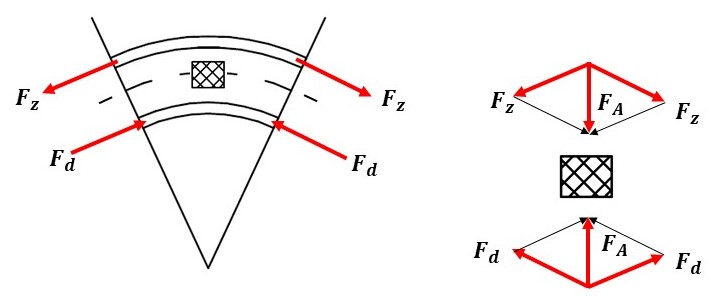
\includegraphics[width=1.0\textwidth]{Bilder/Abtriebskraft.jpg}
	\caption{Prinzip der Druckkraft auf den Steg}
	\label{fig: Abtriebskraft}
\end{figure}
\noindent Darüber hinaus erfährt der Steg einen Schubkraftfluss durch die Querkraft. Wegen der vernachlässigbaren Längskraftaufnahme des Steges im Vergleich zu den Gurten, kann der Schubfluss über die Höhe des Steges als konstant angenommen werden. Die VDI-Richtlinie orientiert sich hier an den Idealisierungen der Schubfeldtheorie, wie sie im entsprechenden Kapitel in \cite{item15} ausgeführt wird. Es muss berücksichtigt werden, dass die Modellierung des Holmes als Balken, der an zwei Punkten gelagert ist und durch die Querkraftbolzen eine weitere Kraft erfährt, zu einem anderen Querkraftverlauf führt als dem konstanten, der in der Richtlinie für den Kragbalken angenommen wurde. Den Berechnungen des Holms als Biegebalken kann für eine Kraft $ F_{pruef}=500N $ eine maximale Querkraft von $ Q_{I}=5085,5N $ im Bereich $ I $ und eine betragsmäßig maximale Querkraft von $Q_{III}=500N $ im Bereich $ III $ entnommen werden. Mit dem Ziel, im langen Bereich $ III $ Gewicht einzusparen, ist es vorteilhaft diesen Bereich geringer Querkraft getrennt von dem höher beanspruchten Bereich $ I $ auszulegen. Der resultierende Schubfluss berechnet sich mithilfe der folgenden Formel:\\
\begin{equation}
	q_{s||}=q_{s}=\frac{Q}{h_{i}} 
\end{equation}
Der gesamte Kraftfluss, der durch den Steg aufgenommen werden muss, ergibt sich dann aus der Überlagerung der drei Kraftflüsse $q_{s||}, n_{A||}, n_{\epsilon||} $. 

\begin{equation}
	n\cdot \bar{q}\cdot K_{\sigma d}\cdot k_{||}=q_{s||}+n_{A||}+n_{\epsilon||} 
\end{equation}

\noindent Die Tragfähigkeit einer Schicht des Verbundes unter Druckbeanspruchung wird durch $ K_{\sigma d} $ charakterisiert und kann ebenfalls Tafel 3 der VDI entnommen werden. An dieser Stelle geht die Richtlinie davon aus, dass die Druckfestigkeit des Laminats im Allgemeinen geringer ist als die Zugfestigkeit. Im vorliegenden Fall zeigen die gegebenen Materialkennwerte des Laminats, dass die Druckfestigkeiten $ R_{||}^{-} $ und $ R_{\perp}^{-} $ deutlich größer als die Zugfestigkeiten $ R_{||}^{+} $, bzw. $ R_{\perp}^{+} $ sind. Dies begründet die Vermutung, dass die vorgestellten Dimensionierungswerte nur für die Vorauslegung auf den vorliegenden Fall übertragbar sind. Da ein Teil der Schubbeanspruchung durch die Matrix geleitet wird, besteht die Gefahr eines Zwischenfaserbruches. VDI 2013 schlägt deshalb die Verwendung von $ K_{\sigma d}=30*10^{3}m $ vor. Zusätzlich muss der Anteil der Glasmengen in Kette und Schuß durch den Faktor $ k_{||} $ berücksichtigt werden. Das zur Verfügung stehende Gewebe Interglas 90070 hat annähernd gleiche Fadenanzahlen und Garnarten in Kette- und Schußrichtung (\cite{item18}), damit ist $ k_{||}=0,5 $. Die Anzahl der notwendigen Gewebelagen n im Steg lässt sich nun durch Umstellen der Gleichungen und Einsetzen der bekannten Werte ermitteln:\\

\begin{equation}
	n=\frac{\frac{2\cdot F_{Pruef}\cdot l_{3}\cdot \epsilon_{Gurt}}{h_{m}^{2}\cdot 2}+\frac{Q}{h_{i}}}{\bar{q}\cdot \left(k_{||}\cdot K_{\sigma d}-K_{E\#}\cdot \epsilon_{Gurt}\cdot 0,5\right)}
\end{equation}
Damit ergibt sich die Lagenanzahl bei einer Prüfrkraft $ F_{pruef}=500N $ von $ n\left(500N\right)=1,99 $ für den Bereich $ 3 $ und $ n\left(5085,5N\right)=18,13 $ für den Bereich $ 1 $. Bereich $ 2 $ erfährt eine Querkraft von $Q_{2}=0N $. Da dieser Bereich sehr kurz ist, wird er so wie Bereich $ 1 $ belegt. Um einen symmetrischen Lagenaufbau im Falle einer Sandwichkonstruktion zu ermöglichen, sind also $ 2 $ Lagen für den Bereich $ 3 $ und $ 20 $ Lagen für die Bereiche $ 1 $ und $ 2 $ vorzusehen.\\

\noindent Es ist zu betonen, dass diese Lagenanzahlen maßgeblich durch die Annahmen der Dimensionierungskennwerte $ K_{E\#} $ und $ K_{\sigma d} $ beeinflusst werden. Da sie als nur beschränkt gültig für den vorliegenden Fall angenommen werden, bedarf es einer aufbauenden Berechnung, die unter anderem die Sicherheiten gegen Zwischenfaserbruch bestimmen kann. Im Kapitel \ref{Puck} wird die hier ermittelte Lagenanzahl mit tatsächlichen Laminatkennwerten und einem Laminatrechner überprüft und angepasst.\\
